\lab{Algorithms}{Crime Mapping}{Crime Mapping}
\objective{Use Gaussian Mixture Models and Kernel Density Estimates to map homicides in Baltimore.}

Suppose we are moving to Baltimore, and we need to find a place to live. We would like to be aware of the crime (homicides in particular) in each neighborhood, as this will certainly influence our decision. We could simply look at a map of all homicides in the city over several years, as shown in Figure \ref{fig:baltimorehomicides}.

\begin{figure}[h]
\centering
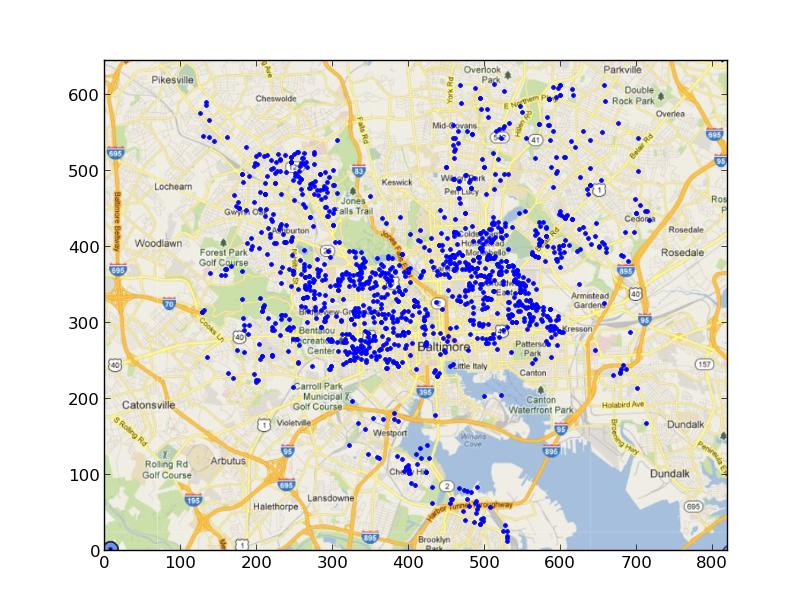
\includegraphics[width=\textwidth]{baltimorecrimemap.jpeg}
\caption{Map of homicides in Baltimore over several years.}
\label{fig:baltimorehomicides}
\end{figure}

This is helpful, but we would like to find the largest geographical area of Baltimore from which to choose a home, with only a small fraction (say $5\%$) of the homicides. This is equivalent to finding the smallest geographical area of Baltimore containing $95\%$ of all homicides. To do this, we'll need to estimate the probability density of homicides in Baltimore.

We will use two approaches to estimating this pdf. The first is via GMMs.

\begin{problem}
Unpickle the file \texttt{homicides}, which contains the approximate longitude (first column) and latitude (second column) of a homicide in Baltimore. Train a $3$-component GMM on this data set.
\end{problem}

We can plot this density over the Baltimore region as in the previous lab, using \li{matplotlib.pyplot.imshow}.

\begin{problem}
Compute the density at each point on a sufficiently fine grid of the Baltimore region. Save a plot of this pdf.
\end{problem}

From this model, we can get a more probabilistic viewpoint of crime in the Baltimore area, as in Figure \ref{fig:baltimoregmm}.

\begin{figure}[h]
\centering
\includegraphics[width=\textwidth]{baltimoregmm.png}
\caption{GMM density over the Baltimore region.}
\label{fig:baltimoregmm}
\end{figure}

Alternatively, we can use a Kernel Density Estimate (KDE) of our data. A KDE is a method of smoothing data. We initially examined a scatterplot of the homicide data. Suppose that given $N$ data points, we replace each data point $x_{i}$ with some symmetric probability distribution $K_{h}$. We call this distribution $K_{h}$ a \emph{kernel}, and it is centered at the origin and has some smoothing parameter $h$. If we scale each kernel by $\frac{1}{N}$, then their sum will be a probability distribution. Thus the KDE for the data $x_{1}, \cdots, x_{n}$ is
\begin{equation*}
\widehat{f}_{h}(x) = \frac{1}{n} \sum_{i=1}^{n} K_{h}(x - x_{i}) = \frac{1}{nh} \sum_{i=1}^{n} K(\frac{x - x_{i}}{h})
\end{equation*}
This formulation allows us to choose a kernel family $K$, and then alter it with a smoothing parameter $h$ to get various kernels. Of course, this formulation only makes sense for univariate data (otherwise $h$ couldn't simply be a scalar).

Choosing $h$ is often the most challenging aspect of dealing with KDEs. If $h$ is chosen too small, then the pdf becomes too multimodal (a large mode at each data point). If it is too large, it is too smooth, approaching a uniform distribution. For univariate data with a Gaussian kernel, an optimal choice for the bandwidth is $h \approx 1.06\widehat{\sigma}n^{-1/5}$ where here, $\widehat{\sigma}$ is the standard deviation of our data.

For multivariate data, the KDE is 
\begin{equation*}
\widehat{f}_{\mathbf{H}}(x) = \frac{1}{n} \sum_{i=1}^{n} K_{\mathbf{H}}(x - x_{i}) = \frac{1}{n\lvert \mathbf{H} \rvert^{\frac{1}{2}}} \sum_{i=1}^{n} K(\mathbf{H}^{-\frac{1}{2}}(x - x_{i}))
\end{equation*}
where $\mathbf{H}$ is a bandwidth matrix, and $K$ is some multivariate symmetric density centered at the origin. Choosing $\mathbf{H}$ is even more difficult in the multivariate case, but a decent results can be obtained by choosing the diagonal matrix $\mathbf{H}$ where 
\begin{equation*}
H_{ii} = (\frac{4}{d+2})^{\frac{2}{d+4}} n^{\frac{-2}{d+4}} \widehat{\sigma}_{i}^{2}
\end{equation*}
where $d$ is the dimension of the data, and $\widehat{\sigma}_{i}$ is the standard deviation of the $i^{th}$ dimension. We will use \li{scipy}'s implementation of the KDE.

The \li{gaussian\_kde} class is initialized with data where each column is a sample, the number of rows being the dimension of the space, and the number of columns being the number of samples. We can evaluate the density of a new sample using the method \li{evaluate}.
\begin{lstlisting}
: import scipy as sp
: from scipy import stats
: kernel = stats.gaussian_kde(data)
: print kernel.evaluate(sp.zeros(data.shape[0]))
\end{lstlisting}

\begin{problem}
Using \li{stats.gaussian\_kde}, initialize a KDE with the homicide data (make sure it's in the right format!), and compute the KDE of each point on your grid of Baltimore. Plot the density and save your plot.
\end{problem}

With this approach, we can get an alternative (and likely better) probabilistic view of crime in Baltimore, as shown in Figure \ref{fig:baltimorekde}.

\begin{figure}[h]
\centering
\includegraphics[width=\textwidth]{baltimorekde.png}
\caption{KDE over the Baltimore region.}
\label{fig:baltimorekde}
\end{figure}

We must still solve the initial problem, i.e. find the smallest geographical area of Baltimore containing $95\%$ of all homicides. We do this by ``vertically integrating'' our densities. In other words, we choose some threshold $t$, find all points $x$ on our grid such that $\widehat{f}_{\mathbf{H}}(x) \geq t$, and compute the integral of our KDE over this region. If the length of each side for each square of our grid is $h$, then we can estimate this integral by
\begin{equation*}
\sum_{x : \widehat{f}_{\mathbf{H}}(x) > t} \widehat{f}_{\mathbf{H}}(x)\cdot h^{2}
\end{equation*}
Ultimately, we are trying to find the region where this integral is approximately $0.95$. Since $t$ is the only thing we can vary, this becomes an optimization problem over $t$, where we are minimizing the objective function
\begin{equation*}
g(t) = \abs{\sum_{x : \widehat{f}_{\mathbf{H}}(x) > t} \widehat{f}_{\mathbf{H}}(x)\cdot h^{2} - 0.95}
\end{equation*}

\begin{problem}
Find this $95\%$ region for both the GMM and the KDE and plot it using \li{imshow}, where each ``safe'' point on the grid is $0$ and each ``unsafe'' region is $1$.
%these final plots are included in the folder with the lab.
\end{problem}
